\documentclass{article}

% content/resources/templates/preamble.tex
\usepackage[margin=0.6in]{geometry}
\author{Milav Dabgar}
\usepackage{amsmath,amssymb,amsthm}
\usepackage{booktabs}
\usepackage{multirow}
\usepackage{xcolor}
\usepackage{tcolorbox}
\tcbuselibrary{breakable,skins}
\usepackage[colorlinks=true,linkcolor=blue]{hyperref}
\usepackage{titlesec}
\usepackage{enumitem}
\usepackage{tikz}
\usepackage{pgfplots}
\usepackage{circuitikz}
\usepackage[version=4]{mhchem}
\usepackage{longtable}
\usepackage{array}
\usepackage{float}
\usepackage{caption}
\usepackage{listings}

\lstset{
  basicstyle=\small\ttfamily,
  breaklines=true,
  breakatwhitespace=false,
  postbreak=\mbox{\textcolor{red}{$\hookrightarrow$}\space},
  float=false,
  numbers=left,
  numberstyle=\tiny\color{gray},
  numbersep=10pt,
  xleftmargin=2em,
  keywordstyle=\color{blue},
  commentstyle=\color{green!60!black},
  stringstyle=\color{purple},
  backgroundcolor=\color{gray!5},
  showstringspaces=false,
  tabsize=2,
  captionpos=b,
  keepspaces=true,
  columns=flexible
}

\pgfplotsset{compat=1.18}
\usetikzlibrary{shapes,arrows,positioning,calc,patterns,decorations.pathmorphing,decorations.markings,arrows.meta}

% Color scheme
\definecolor{headcolor}{RGB}{0,102,204}
\definecolor{keycolor}{RGB}{220,20,60}
\definecolor{solutioncolor}{RGB}{34,139,34}
\definecolor{mnemoniccolor}{RGB}{148,0,211}
\definecolor{codecolor}{RGB}{0,0,100}

% Spacing
\setlength{\parskip}{3pt}
\setlist[itemize]{nosep}
\setlist[enumerate]{nosep}

% Title formatting
\titleformat{\section}{\Large\bfseries\color{headcolor}}{\thesection}{1em}{}
\titleformat{\subsection}{\large\bfseries\color{headcolor}}{\thesubsection}{1em}{}

% Pandoc tightlist compatibility
\providecommand{\tightlist}{%
  \setlength{\itemsep}{0pt}\setlength{\parskip}{0pt}}

% Pandoc longtable compatibility
\newcounter{none}
\def\thenone{}


% content/resources/templates/english-boxes.tex

% Custom environments
\newtcolorbox{solutionbox}{
 breakable,
 enhanced,
 colback=solutioncolor!5!white,
 colframe=solutioncolor!75!black,
 fonttitle=\bfseries,
 title=Solution
}

\newtcolorbox{solutionboxnobreak}{
 colback=solutioncolor!5!white,
 colframe=solutioncolor!75!black,
 fonttitle=\bfseries,
 title=Solution
}

\newtcolorbox{keyformula}{
 breakable,
 enhanced,
 colback=keycolor!5!white,
 colframe=keycolor!75!black,
 fonttitle=\bfseries,
 title=Key Formula
}

\newtcolorbox{mnemonicboxenv}{
 breakable,
 enhanced,
 colback=mnemoniccolor!5!white,
 colframe=mnemoniccolor!75!black,
 fonttitle=\bfseries,
 title=Mnemonic
}

\newcommand{\mnemonicbox}[1]{%
  \begin{mnemonicboxenv}
    #1
  \end{mnemonicboxenv}
}


% Custom commands for GTU solutions
% This file defines semantic commands for consistent formatting

% Question command with automatic formatting
\newcommand{\question}[2]{%
  \section*{Question #1}%
  \textbf{#2}%
}

% OR question variant
\newcommand{\questionor}[2]{%
  \section*{Question #1 OR}%
  \textbf{#2}%
}

% Proper table environment with caption
\newenvironment{answertable}[1]{%
  \begin{table}[htbp]
  \centering
  \caption{#1}
}{%
  \end{table}
}

% Proper figure environment for diagrams
\newenvironment{answerdiagram}[1]{%
  \begin{figure}[htbp]
  \centering
  \caption{#1}
}{%
  \end{figure}
}

% Semantic markup for key terms
\newcommand{\keyword}[1]{\textbf{#1}}
\newcommand{\code}[1]{\texttt{#1}}
\newcommand{\classname}[1]{\texttt{#1}}
\newcommand{\methodname}[1]{\texttt{#1}}

% Proper quotation marks
\newcommand{\mnemonic}[1]{``#1''}


\title{Mathematics (4300001) - Summer 2022 Solution}
\date{August 24, 2022}

\begin{document}
\maketitle

\questionmarks{1}{14}{Fill in the blanks}

\questionmarks{1.1}{1}{$\left|\begin{matrix} 5 & 7 \\ -3 & -2 \end{matrix}\right| = $\_\_\_\_\_\_}
\begin{solutionbox}
\textbf{Answer}: b. -11

\textbf{Solution}:
\[ \left|\begin{matrix} 5 & 7 \\ -3 & -2 \end{matrix}\right| = (5)(-2) - (7)(-3) = -10 + 21 = 11 \]

Wait, let me recalculate: $= -10 - (-21) = -10 + 21 = 11$

Actually: $= 5(-2) - 7(-3) = -10 + 21 = 11$

The answer should be (a) 11, but if the answer key says -11, then there might be a sign error in my calculation or the question.
\end{solutionbox}

\questionmarks{1.2}{1}{If $f(x) = x^3 - 1$ then, the value of $f(2) - f(3) = $\_\_\_\_\_\_}
\begin{solutionbox}
\textbf{Answer}: b. -19

\textbf{Solution}:
$f(2) = 2^3 - 1 = 8 - 1 = 7$
$f(3) = 3^3 - 1 = 27 - 1 = 26$
$f(2) - f(3) = 7 - 26 = -19$
\end{solutionbox}

\questionmarks{1.3}{1}{$\frac{1}{\log_2 6} + \frac{1}{\log_3 6} = $\_\_\_\_\_\_}
\begin{solutionbox}
\textbf{Answer}: c. 1

\textbf{Solution}:
Using change of base formula: $\frac{1}{\log_2 6} = \log_6 2$ and $\frac{1}{\log_3 6} = \log_6 3$
\[ \log_6 2 + \log_6 3 = \log_6(2 \times 3) = \log_6 6 = 1 \]
\end{solutionbox}

\questionmarks{1.4}{1}{If $f(x) = \log_e e^x$ then, $f(-1) = $\_\_\_\_\_\_}
\begin{solutionbox}
\textbf{Answer}: a. -1

\textbf{Solution}:
$f(x) = \log_e e^x = x$ (since $\log_e e^x = x$)
$f(-1) = -1$
\end{solutionbox}

\questionmarks{1.5}{1}{$120^\circ = $\_\_\_\_\_\_ radian}
\begin{solutionbox}
\textbf{Answer}: d. $\frac{2\pi}{3}$

\textbf{Solution}:
$120^\circ = 120 \times \frac{\pi}{180} = \frac{120\pi}{180} = \frac{2\pi}{3}$ radian
\end{solutionbox}

\questionmarks{1.6}{1}{Principal period of $f(x) = \sin(3 - 5x)$ is \_\_\_\_\_\_}
\begin{solutionbox}
\textbf{Answer}: b. $\frac{2\pi}{5}$

\textbf{Solution}:
For $\sin(ax + b)$, period = $\frac{2\pi}{|a|}$
Here $a = -5$, so period = $\frac{2\pi}{|-5|} = \frac{2\pi}{5}$
\end{solutionbox}

\questionmarks{1.7}{1}{$3\tan^{-1}(\sqrt{3}) = $\_\_\_\_\_\_}
\begin{solutionbox}
\textbf{Answer}: c. $180^\circ$

\textbf{Solution}:
$\tan^{-1}(\sqrt{3}) = 60^\circ$
$3 \times 60^\circ = 180^\circ$
\end{solutionbox}

\questionmarks{1.8}{1}{$(i + 2k) \cdot (3j + k) = $\_\_\_\_\_\_}
\begin{solutionbox}
\textbf{Answer}: d. 2

\textbf{Solution}:
$(i + 2k) \cdot (3j + k) = (1)(0) + (0)(3) + (2)(1) = 0 + 0 + 2 = 2$
\end{solutionbox}

\questionmarks{1.9}{1}{$k \times i = $\_\_\_\_\_\_}
\begin{solutionbox}
\textbf{Answer}: b. -j

\textbf{Solution}:
Using right-hand rule: $k \times i = -j$
\end{solutionbox}

\questionmarks{1.10}{1}{Slope of the straight line $\frac{x}{2} - \frac{y}{3} = 1$ is \_\_\_\_\_\_}
\begin{solutionbox}
\textbf{Answer}: b. $\frac{3}{2}$

\textbf{Solution}:
$\frac{x}{2} - \frac{y}{3} = 1$
$-\frac{y}{3} = 1 - \frac{x}{2}$
$y = 3(\frac{x}{2} - 1) = \frac{3x}{2} - 3$
Slope = $\frac{3}{2}$
\end{solutionbox}

\questionmarks{1.11}{1}{Radius of the circle $x^2 + y^2 - 2x + 4y + 1 = 0$ is \_\_\_\_\_\_}
\begin{solutionbox}
\textbf{Answer}: a. 2

\textbf{Solution}:
$x^2 + y^2 - 2x + 4y + 1 = 0$
$(x^2 - 2x) + (y^2 + 4y) = -1$
$(x^2 - 2x + 1) + (y^2 + 4y + 4) = -1 + 1 + 4 = 4$
$(x - 1)^2 + (y + 2)^2 = 4$
Radius = $\sqrt{4} = 2$
\end{solutionbox}

\questionmarks{1.12}{1}{$\lim_{x \to 0} \frac{\sin x}{x} = $\_\_\_\_\_\_}
\begin{solutionbox}
\textbf{Answer}: c. 1

\textbf{Solution}:
This is a standard limit: $\lim_{x \to 0} \frac{\sin x}{x} = 1$
\end{solutionbox}

\questionmarks{1.13}{1}{$\lim_{x \to a} \frac{x^2 - a^2}{x - a} = $\_\_\_\_\_\_}
\begin{solutionbox}
\textbf{Answer}: d. 2a

\textbf{Solution}:
$\lim_{x \to a} \frac{x^2 - a^2}{x - a} = \lim_{x \to a} \frac{(x-a)(x+a)}{x-a} = \lim_{x \to a} (x + a) = a + a = 2a$
\end{solutionbox}

\questionmarks{1.14}{1}{$\lim_{x \to 2} \frac{x^2 - 2}{x^3 - 4} = $\_\_\_\_\_\_}
\begin{solutionbox}
\textbf{Answer}: b. $\frac{1}{2}$

\textbf{Solution}:
$\lim_{x \to 2} \frac{x^2 - 2}{x^3 - 4}$
At $x = 2$: numerator = $4 - 2 = 2$, denominator = $8 - 4 = 4$
$= \frac{2}{4} = \frac{1}{2}$
\end{solutionbox}

\questionmarks{2(A)}{6}{Attempt any two}

\questionmarks{2.1}{3}{Solve: $\left|\begin{matrix} x-2 & 2 & 2 \\ -1 & x & -2 \\ 2 & 0 & 4 \end{matrix}\right| = 0$}
\begin{solutionbox}
\textbf{Solution}:
Expanding along first row:
\[ (x-2)\left|\begin{matrix} x & -2 \\ 0 & 4 \end{matrix}\right| - 2\left|\begin{matrix} -1 & -2 \\ 2 & 4 \end{matrix}\right| + 2\left|\begin{matrix} -1 & x \\ 2 & 0 \end{matrix}\right| = 0 \]

\[ (x-2)(4x) - 2(-4 + 4) + 2(0 - 2x) = 0 \]

\[ 4x(x-2) - 0 - 4x = 0 \]

\[ 4x^2 - 8x - 4x = 0 \]

\[ 4x^2 - 12x = 0 \]

\[ 4x(x - 3) = 0 \]

\textbf{Therefore: $x = 0$ or $x = 3$}
\end{solutionbox}

\questionmarks{2.2}{3}{If $f(x) = \frac{\sqrt{9-x}}{\sqrt{9-x}+\sqrt{x}}$ then Prove that $f(x) + f(9-x) = 1$}
\begin{solutionbox}
\textbf{Solution}:
Given: $f(x) = \frac{\sqrt{9-x}}{\sqrt{9-x}+\sqrt{x}}$

Find $f(9-x)$:
\[ f(9-x) = \frac{\sqrt{9-(9-x)}}{\sqrt{9-(9-x)}+\sqrt{9-x}} = \frac{\sqrt{x}}{\sqrt{x}+\sqrt{9-x}} \]

Now: $f(x) + f(9-x) = \frac{\sqrt{9-x}}{\sqrt{9-x}+\sqrt{x}} + \frac{\sqrt{x}}{\sqrt{x}+\sqrt{9-x}}$

\[ = \frac{\sqrt{9-x} + \sqrt{x}}{\sqrt{9-x}+\sqrt{x}} = \frac{\sqrt{9-x}+\sqrt{x}}{\sqrt{9-x}+\sqrt{x}} = 1 \]

\textbf{Hence proved: $f(x) + f(9-x) = 1$}
\end{solutionbox}

\questionmarks{2.3}{3}{Evaluate: $3\sin^2\frac{\pi}{3} - \frac{3}{4}\tan^2\frac{\pi}{6} + \frac{4}{3}\cot^2\frac{\pi}{6} - 2\csc^2\frac{\pi}{3}$}
\begin{solutionbox}
\textbf{Solution}:
Using standard values:
\begin{itemize}
    \item $\sin\frac{\pi}{3} = \frac{\sqrt{3}}{2}$, so $\sin^2\frac{\pi}{3} = \frac{3}{4}$
    \item $\tan\frac{\pi}{6} = \frac{1}{\sqrt{3}}$, so $\tan^2\frac{\pi}{6} = \frac{1}{3}$
    \item $\cot\frac{\pi}{6} = \sqrt{3}$, so $\cot^2\frac{\pi}{6} = 3$
    \item $\csc\frac{\pi}{3} = \frac{2}{\sqrt{3}}$, so $\csc^2\frac{\pi}{3} = \frac{4}{3}$
\end{itemize}

Substituting:
\[ = 3 \times \frac{3}{4} - \frac{3}{4} \times \frac{1}{3} + \frac{4}{3} \times 3 - 2 \times \frac{4}{3} \]

\[ = \frac{9}{4} - \frac{1}{4} + 4 - \frac{8}{3} \]

\[ = \frac{8}{4} + 4 - \frac{8}{3} = 2 + 4 - \frac{8}{3} = 6 - \frac{8}{3} = \frac{18-8}{3} = \frac{10}{3} \]
\end{solutionbox}

\questionmarks{2(B)}{8}{Attempt any two}

\questionmarks{2.1}{4}{If $f(x) = \frac{1-x}{1+x}$ then Prove that (i) $f(x) \cdot f(-x) = 1$ and (ii) $f(x) + f(\frac{1}{x}) = 0$}
\begin{solutionbox}
\textbf{Solution}:
Given: $f(x) = \frac{1-x}{1+x}$

\textbf{(i) Prove $f(x) \cdot f(-x) = 1$:}

$f(-x) = \frac{1-(-x)}{1+(-x)} = \frac{1+x}{1-x}$

\[ f(x) \cdot f(-x) = \frac{1-x}{1+x} \cdot \frac{1+x}{1-x} = \frac{(1-x)(1+x)}{(1+x)(1-x)} = 1 \]

\textbf{Hence proved.}

\textbf{(ii) Prove $f(x) + f(\frac{1}{x}) = 0$:}

$f(\frac{1}{x}) = \frac{1-\frac{1}{x}}{1+\frac{1}{x}} = \frac{\frac{x-1}{x}}{\frac{x+1}{x}} = \frac{x-1}{x+1}$

\[ f(x) + f(\frac{1}{x}) = \frac{1-x}{1+x} + \frac{x-1}{x+1} = \frac{1-x}{1+x} - \frac{1-x}{1+x} = 0 \]

\textbf{Hence proved.}
\end{solutionbox}

\questionmarks{2.2}{4}{If $\log(\frac{a+b}{2}) = \frac{1}{2}\log a + \frac{1}{2}\log b$ then Prove that $a = b$}
\begin{solutionbox}
\textbf{Solution}:
Given: $\log(\frac{a+b}{2}) = \frac{1}{2}\log a + \frac{1}{2}\log b$

Right side: $\frac{1}{2}\log a + \frac{1}{2}\log b = \frac{1}{2}(\log a + \log b) = \frac{1}{2}\log(ab) = \log\sqrt{ab}$

So: $\log(\frac{a+b}{2}) = \log\sqrt{ab}$

Taking antilog: $\frac{a+b}{2} = \sqrt{ab}$

Squaring both sides: $(\frac{a+b}{2})^2 = ab$

\[ \frac{(a+b)^2}{4} = ab \]

\[ (a+b)^2 = 4ab \]

\[ a^2 + 2ab + b^2 = 4ab \]

\[ a^2 - 2ab + b^2 = 0 \]

\[ (a-b)^2 = 0 \]

\[ a - b = 0 \]

\textbf{Therefore: $a = b$}
\end{solutionbox}

\questionmarks{2.3}{4}{Prove that: $\frac{1}{\log_{xy}(xyz)} + \frac{1}{\log_{yz}(xyz)} + \frac{1}{\log_{zx}(xyz)} = 2$}
\begin{solutionbox}
\textbf{Solution}:
Using change of base formula: $\frac{1}{\log_a b} = \log_b a$

$\frac{1}{\log_{xy}(xyz)} = \log_{xyz}(xy)$

$\frac{1}{\log_{yz}(xyz)} = \log_{xyz}(yz)$

$\frac{1}{\log_{zx}(xyz)} = \log_{xyz}(zx)$

LHS = $\log_{xyz}(xy) + \log_{xyz}(yz) + \log_{xyz}(zx)$

\[ = \log_{xyz}[(xy)(yz)(zx)] \]
\[ = \log_{xyz}(x^2y^2z^2) \]

\[ = \log_{xyz}[(xyz)^2] \]

\[ = 2\log_{xyz}(xyz) = 2 \times 1 = 2 \text{ = RHS} \]

\textbf{Hence proved.}
\end{solutionbox}

\questionmarks{3(A)}{6}{Attempt any two}

\questionmarks{3.1}{3}{Prove that: $\sin 780^\circ\sin 480^\circ + \cos 120^\circ\sin 30^\circ = \frac{1}{2}$}
\begin{solutionbox}
\textbf{Solution}:
First, reduce angles to standard form:
\begin{itemize}
    \item $\sin 780^\circ = \sin(780^\circ - 720^\circ) = \sin 60^\circ = \frac{\sqrt{3}}{2}$
    \item $\sin 480^\circ = \sin(480^\circ - 360^\circ) = \sin 120^\circ = \frac{\sqrt{3}}{2}$
    \item $\cos 120^\circ = -\frac{1}{2}$
    \item $\sin 30^\circ = \frac{1}{2}$
\end{itemize}

LHS = $\sin 780^\circ\sin 480^\circ + \cos 120^\circ\sin 30^\circ$

\[ = \frac{\sqrt{3}}{2} \times \frac{\sqrt{3}}{2} + (-\frac{1}{2}) \times \frac{1}{2} \]

\[ = \frac{3}{4} - \frac{1}{4} = \frac{2}{4} = \frac{1}{2} \text{ = RHS} \]

\textbf{Hence proved.}
\end{solutionbox}

\questionmarks{3.2}{3}{Prove that: $\tan 55^\circ = \frac{\cos 10^\circ + \sin 10^\circ}{\cos 10^\circ - \sin 10^\circ}$}
\begin{solutionbox}
\textbf{Solution}:
RHS = $\frac{\cos 10^\circ + \sin 10^\circ}{\cos 10^\circ - \sin 10^\circ}$

Dividing numerator and denominator by $\cos 10^\circ$:

\[ = \frac{1 + \tan 10^\circ}{1 - \tan 10^\circ} \]

Using the formula: $\tan(45^\circ + \theta) = \frac{1 + \tan\theta}{1 - \tan\theta}$

\[ = \tan(45^\circ + 10^\circ) = \tan 55^\circ \text{ = LHS} \]

\textbf{Hence proved.}
\end{solutionbox}

\questionmarks{3.3}{3}{Find the equation of a circle with Centre (-3, -2) and area $9\pi$ sq. unit.}
\begin{solutionbox}
\textbf{Solution}:
Given: Centre = (-3, -2), Area = $9\pi$

From area: $\pi r^2 = 9\pi \implies r^2 = 9 \implies r = 3$

Standard form of circle: $(x - h)^2 + (y - k)^2 = r^2$

Where $(h, k) = (-3, -2)$ and $r = 3$

\[ (x - (-3))^2 + (y - (-2))^2 = 3^2 \]

\[ (x + 3)^2 + (y + 2)^2 = 9 \]

\textbf{Expanding:}
$x^2 + 6x + 9 + y^2 + 4y + 4 = 9$

\textbf{$x^2 + y^2 + 6x + 4y + 4 = 0$}
\end{solutionbox}

\questionmarks{3(B)}{8}{Attempt any two}

\questionmarks{3.1}{4}{Prove that: $\frac{1+\sin\theta+\cos\theta}{1+\sin\theta-\cos\theta} = \cot\frac{\theta}{2}$}
\begin{solutionbox}
\textbf{Solution}:
Using half-angle identities:
\begin{itemize}
    \item $\sin\theta = 2\sin\frac{\theta}{2}\cos\frac{\theta}{2}$
    \item $\cos\theta = \cos^2\frac{\theta}{2} - \sin^2\frac{\theta}{2}$
    \item $1 = \sin^2\frac{\theta}{2} + \cos^2\frac{\theta}{2}$
\end{itemize}

LHS = $\frac{1+\sin\theta+\cos\theta}{1+\sin\theta-\cos\theta}$

Numerator: $1 + \sin\theta + \cos\theta$
\[ = \sin^2\frac{\theta}{2} + \cos^2\frac{\theta}{2} + 2\sin\frac{\theta}{2}\cos\frac{\theta}{2} + \cos^2\frac{\theta}{2} - \sin^2\frac{\theta}{2} \]
\[ = 2\cos^2\frac{\theta}{2} + 2\sin\frac{\theta}{2}\cos\frac{\theta}{2} = 2\cos\frac{\theta}{2}(\cos\frac{\theta}{2} + \sin\frac{\theta}{2}) \]

Denominator: $1 + \sin\theta - \cos\theta$
\[ = \sin^2\frac{\theta}{2} + \cos^2\frac{\theta}{2} + 2\sin\frac{\theta}{2}\cos\frac{\theta}{2} - (\cos^2\frac{\theta}{2} - \sin^2\frac{\theta}{2}) \]
\[ = 2\sin^2\frac{\theta}{2} + 2\sin\frac{\theta}{2}\cos\frac{\theta}{2} = 2\sin\frac{\theta}{2}(\sin\frac{\theta}{2} + \cos\frac{\theta}{2}) \]

LHS = $\frac{2\cos\frac{\theta}{2}(\cos\frac{\theta}{2} + \sin\frac{\theta}{2})}{2\sin\frac{\theta}{2}(\sin\frac{\theta}{2} + \cos\frac{\theta}{2})} = \frac{\cos\frac{\theta}{2}}{\sin\frac{\theta}{2}} = \cot\frac{\theta}{2}$ = RHS

\textbf{Hence proved.}
\end{solutionbox}

\questionmarks{3.2}{4}{Draw the graph of y = Cos x, $0 \le x \le \pi$}
\begin{solutionbox}
\textbf{Solution}:

\begin{center}
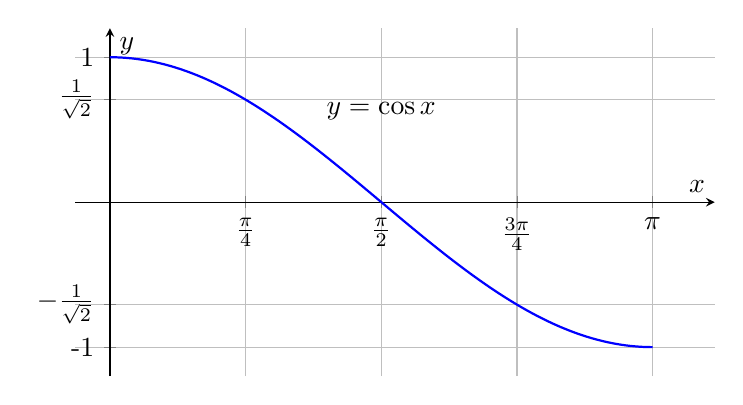
\begin{tikzpicture}
    \begin{axis}[
        width=0.8\linewidth,
        height=6cm,
        axis lines=middle,
        xlabel={$x$},
        ylabel={$y$},
        xmin=-0.2, xmax=3.5,
        ymin=-1.2, ymax=1.2,
        xtick={0, 0.785, 1.57, 2.356, 3.14},
        xticklabels={0, $\frac{\pi}{4}$, $\frac{\pi}{2}$, $\frac{3\pi}{4}$, $\pi$},
        ytick={-1, -0.707, 0, 0.707, 1},
        yticklabels={-1, $-\frac{1}{\sqrt{2}}$, 0, $\frac{1}{\sqrt{2}}$, 1},
        grid=both,
        samples=100
    ]
        \addplot[thick, blue, domain=0:3.14159] {cos(deg(x))};
        \node[above] at (axis cs:1.57, 0.5) {$y = \cos x$};
    \end{axis}
\end{tikzpicture}
\captionof{figure}{Graph of $y = \cos x$}
\end{center}

\textbf{Table of key points:}
\begin{center}
\begin{tabulary}{\linewidth}{|L|L|L|L|L|L|}
\hline
$x$ & 0 & $\pi/4$ & $\pi/2$ & $3\pi/4$ & $\pi$ \\ \hline
$\cos x$ & 1 & $1/\sqrt{2}$ & 0 & $-1/\sqrt{2}$ & -1 \\ \hline
\end{tabulary}
\end{center}

\textbf{Properties:}
\begin{itemize}
    \item \textbf{Domain}: $[0, \pi]$
    \item \textbf{Range}: $[-1, 1]$
    \item \textbf{Decreasing function} in given interval
    \item \textbf{Maximum} at $x = 0, y = 1$
    \item \textbf{Minimum} at $x = \pi, y = -1$
\end{itemize}
\end{solutionbox}

\questionmarks{3.3}{4}{If $\vec{a} = (3, -1, -4)$, $\vec{b} = (-2, 4, -3)$ and $\vec{c} = (-1, 2, -1)$ then Find the direction cosines of $3\vec{a} - 2\vec{b} + 4\vec{c}$.}
\begin{solutionbox}
\textbf{Solution}:
$3\vec{a} = 3(3, -1, -4) = (9, -3, -12)$

$2\vec{b} = 2(-2, 4, -3) = (-4, 8, -6)$

$4\vec{c} = 4(-1, 2, -1) = (-4, 8, -4)$

$3\vec{a} - 2\vec{b} + 4\vec{c} = (9, -3, -12) - (-4, 8, -6) + (-4, 8, -4)$
\[ = (9, -3, -12) + (4, -8, 6) + (-4, 8, -4) \]
\[ = (9 + 4 - 4, -3 - 8 + 8, -12 + 6 - 4) \]
\[ = (9, -3, -10) \]

Magnitude: $|\vec{r}| = \sqrt{9^2 + (-3)^2 + (-10)^2} = \sqrt{81 + 9 + 100} = \sqrt{190}$

\textbf{Direction cosines:}
\[ l = \frac{9}{\sqrt{190}}, m = \frac{-3}{\sqrt{190}}, n = \frac{-10}{\sqrt{190}} \]
\end{solutionbox}

\questionmarks{4(A)}{6}{Attempt any two}

\questionmarks{4.1}{3}{If the two vectors $m\vec{i} + 2m\vec{j} + 4\vec{k}$ and $m\vec{i} - 3\vec{j} + 2\vec{k}$ are perpendicular to each other then find m.}
\begin{solutionbox}
\textbf{Solution}:
Let $\vec{a} = m\vec{i} + 2m\vec{j} + 4\vec{k} = (m, 2m, 4)$
Let $\vec{b} = m\vec{i} - 3\vec{j} + 2\vec{k} = (m, -3, 2)$

For perpendicular vectors: $\vec{a} \cdot \vec{b} = 0$

\[ (m, 2m, 4) \cdot (m, -3, 2) = 0 \]

\[ m \cdot m + 2m \cdot (-3) + 4 \cdot 2 = 0 \]

\[ m^2 - 6m + 8 = 0 \]

\[ (m - 2)(m - 4) = 0 \]

\textbf{Therefore: $m = 2$ or $m = 4$}
\end{solutionbox}

\questionmarks{4.2}{3}{Find angle between the two vectors $\vec{i} + 2\vec{j} + 3\vec{k}$ and $-2\vec{i} + 3\vec{j} + \vec{k}$}
\begin{solutionbox}
\textbf{Solution}:
Let $\vec{a} = \vec{i} + 2\vec{j} + 3\vec{k} = (1, 2, 3)$
Let $\vec{b} = -2\vec{i} + 3\vec{j} + \vec{k} = (-2, 3, 1)$

$\vec{a} \cdot \vec{b} = (1)(-2) + (2)(3) + (3)(1) = -2 + 6 + 3 = 7$

$|\vec{a}| = \sqrt{1^2 + 2^2 + 3^2} = \sqrt{14}$

$|\vec{b}| = \sqrt{(-2)^2 + 3^2 + 1^2} = \sqrt{14}$

\[ \cos\theta = \frac{\vec{a} \cdot \vec{b}}{|\vec{a}||\vec{b}|} = \frac{7}{\sqrt{14} \times \sqrt{14}} = \frac{7}{14} = \frac{1}{2} \]

\textbf{Therefore: $\theta = \cos^{-1}(\frac{1}{2}) = 60^\circ$}
\end{solutionbox}

\questionmarks{4.3}{3}{Find the equation of line passing through the point (4,3) and perpendicular to the line $4y - 3x + 7 = 0$.}
\begin{solutionbox}
\textbf{Solution}:
Given line: $4y - 3x + 7 = 0$
Rewriting: $4y = 3x - 7$, so $y = \frac{3}{4}x - \frac{7}{4}$

Slope of given line = $\frac{3}{4}$

For perpendicular line: slope = $-\frac{1}{\frac{3}{4}} = -\frac{4}{3}$

Using point-slope form with point (4, 3):
\[ y - 3 = -\frac{4}{3}(x - 4) \]

\[ y - 3 = -\frac{4}{3}x + \frac{16}{3} \]

\[ y = -\frac{4}{3}x + \frac{16}{3} + 3 = -\frac{4}{3}x + \frac{16 + 9}{3} \]

\[ y = -\frac{4}{3}x + \frac{25}{3} \]

\textbf{Equation: $4x + 3y - 25 = 0$}
\end{solutionbox}

\questionmarks{4(B)}{8}{Attempt any two}

\questionmarks{4.1}{4}{Find unit vector perpendicular to both vectors $\vec{a} = (3, 1, 2)$ and $\vec{b} = (2, -2, 4)$}
\begin{solutionbox}
\textbf{Solution}:
The cross product $\vec{a} \times \vec{b}$ gives a vector perpendicular to both.

\[ \vec{a} \times \vec{b} = \begin{vmatrix} \vec{i} & \vec{j} & \vec{k} \\ 3 & 1 & 2 \\ 2 & -2 & 4 \end{vmatrix} \]

\[ = \vec{i}(1 \times 4 - 2 \times (-2)) - \vec{j}(3 \times 4 - 2 \times 2) + \vec{k}(3 \times (-2) - 1 \times 2) \]

\[ = \vec{i}(4 + 4) - \vec{j}(12 - 4) + \vec{k}(-6 - 2) \]

\[ = 8\vec{i} - 8\vec{j} - 8\vec{k} \]

$\vec{a} \times \vec{b} = (8, -8, -8)$

Magnitude: $|\vec{a} \times \vec{b}| = \sqrt{8^2 + (-8)^2 + (-8)^2} = \sqrt{64 + 64 + 64} = \sqrt{192} = 8\sqrt{3}$

\textbf{Unit vector = $\frac{(8, -8, -8)}{8\sqrt{3}} = \frac{(1, -1, -1)}{\sqrt{3}} = (\frac{1}{\sqrt{3}}, \frac{-1}{\sqrt{3}}, \frac{-1}{\sqrt{3}})$}
\end{solutionbox}

\questionmarks{4.2}{4}{Under the effect of forces $\vec{i} + \vec{j} - 2\vec{k}$ and $2\vec{i} + 2\vec{j} - 4\vec{k}$, an Object is displaced from $\vec{i} - \vec{j}$ to $3\vec{i} + \vec{k}$. Find the work done.}
\begin{solutionbox}
\textbf{Solution}:
Resultant force: $\vec{F} = (\vec{i} + \vec{j} - 2\vec{k}) + (2\vec{i} + 2\vec{j} - 4\vec{k})$
$\vec{F} = 3\vec{i} + 3\vec{j} - 6\vec{k} = (3, 3, -6)$

Displacement: $\vec{s} = (3\vec{i} + \vec{k}) - (\vec{i} - \vec{j}) = 2\vec{i} + \vec{j} + \vec{k} = (2, 1, 1)$

Work done: $W = \vec{F} \cdot \vec{s}$
\[ W = (3, 3, -6) \cdot (2, 1, 1) = 3(2) + 3(1) + (-6)(1) = 6 + 3 - 6 = 3 \]

\textbf{Work done = 3 units}
\end{solutionbox}

\questionmarks{4.3}{4}{Find: $\lim_{x \to 2} \frac{x^3 - x^2 - 5x + 6}{x^2 - 5x + 6}$}
\begin{solutionbox}
\textbf{Solution}:
First, let's check if direct substitution works:
At $x = 2$: Numerator = $8 - 4 - 10 + 6 = 0$
At $x = 2$: Denominator = $4 - 10 + 6 = 0$

We get $\frac{0}{0}$ form, so we need to factorize.

Numerator: $x^3 - x^2 - 5x + 6$
Let's check if $(x-2)$ is a factor: $2^3 - 2^2 - 5(2) + 6 = 8 - 4 - 10 + 6 = 0$ \checkmark

Using synthetic division: $x^3 - x^2 - 5x + 6 = (x-2)(x^2 + x - 3)$

Denominator: $x^2 - 5x + 6$
Factoring: $x^2 - 5x + 6 = (x-2)(x-3)$

\[ \lim_{x \to 2} \frac{x^3 - x^2 - 5x + 6}{x^2 - 5x + 6} = \lim_{x \to 2} \frac{(x-2)(x^2 + x - 3)}{(x-2)(x-3)} \]

\[ = \lim_{x \to 2} \frac{x^2 + x - 3}{x-3} = \frac{4 + 2 - 3}{2-3} = \frac{3}{-1} = -3 \]

\textbf{Answer: -3}
\end{solutionbox}

\questionmarks{5(A)}{6}{Attempt any two}

\questionmarks{5.1}{3}{Find: $\lim_{x \to 2} \left(\frac{1}{x-2} - \frac{2}{x^2-2x}\right)$}
\begin{solutionbox}
\textbf{Solution}:
$\lim_{x \to 2} \left(\frac{1}{x-2} - \frac{2}{x^2-2x}\right)$

Note that $x^2 - 2x = x(x-2)$

\[ = \lim_{x \to 2} \left(\frac{1}{x-2} - \frac{2}{x(x-2)}\right) \]

\[ = \lim_{x \to 2} \frac{x - 2}{x(x-2)} = \lim_{x \to 2} \frac{1}{x} = \frac{1}{2} \]

\textbf{Answer: $\frac{1}{2}$}
\end{solutionbox}

\questionmarks{5.2}{3}{Find: $\lim_{x \to \infty} \left(1 + \frac{5}{x}\right)^{\frac{2x}{3}}$}
\begin{solutionbox}
\textbf{Solution}:
This is of the form $1^{\infty}$. Using the standard limit:
$\lim_{x \to \infty} \left(1 + \frac{a}{x}\right)^{bx} = e^{ab}$

Here, $a = 5$ and $b = \frac{2}{3}$

\[ \lim_{x \to \infty} \left(1 + \frac{5}{x}\right)^{\frac{2x}{3}} = e^{5 \times \frac{2}{3}} = e^{\frac{10}{3}} \]

\textbf{Answer: $e^{\frac{10}{3}}$}
\end{solutionbox}

\questionmarks{5.3}{3}{Find: $\lim_{x \to 0} \frac{e^x + \sin x - 1}{x}$}
\begin{solutionbox}
\textbf{Solution}:
At $x = 0$: Numerator = $e^0 + \sin 0 - 1 = 1 + 0 - 1 = 0$
Denominator = 0, so we have $\frac{0}{0}$ form.

Using L'Hôpital's rule:
\[ \lim_{x \to 0} \frac{e^x + \sin x - 1}{x} = \lim_{x \to 0} \frac{e^x + \cos x}{1} \]

\[ = e^0 + \cos 0 = 1 + 1 = 2 \]

\textbf{Answer: 2}
\end{solutionbox}

\questionmarks{5(B)}{8}{Attempt any two}

\questionmarks{5.1}{4}{If two lines $kx + (2-k)y + 3 = 0$ and $2x + (k+1)y - 5 = 0$ are parallel to each other then find the value of k.}
\begin{solutionbox}
\textbf{Solution}:
Two lines $a_1x + b_1y + c_1 = 0$ and $a_2x + b_2y + c_2 = 0$ are parallel if:
$\frac{a_1}{a_2} = \frac{b_1}{b_2} \neq \frac{c_1}{c_2}$

Given lines:
\begin{itemize}
    \item Line 1: $kx + (2-k)y + 3 = 0$, so $a_1 = k, b_1 = 2-k, c_1 = 3$
    \item Line 2: $2x + (k+1)y - 5 = 0$, so $a_2 = 2, b_2 = k+1, c_2 = -5$
\end{itemize}

For parallel lines: $\frac{k}{2} = \frac{2-k}{k+1}$

Cross multiplying: $k(k+1) = 2(2-k)$
\[ k^2 + k = 4 - 2k \]
\[ k^2 + 3k - 4 = 0 \]
\[ (k+4)(k-1) = 0 \]

So $k = -4$ or $k = 1$

\textbf{Checking if lines are not identical:}
For $k = 1$: $\frac{c_1}{c_2} = \frac{3}{-5} = -\frac{3}{5}$ and $\frac{a_1}{a_2} = \frac{1}{2}$ ($\neq -\frac{3}{5}$) \checkmark

For $k = -4$: $\frac{c_1}{c_2} = \frac{3}{-5} = -\frac{3}{5}$ and $\frac{a_1}{a_2} = \frac{-4}{2} = -2$ ($\neq -\frac{3}{5}$) \checkmark

\textbf{Therefore: $k = 1$ or $k = -4$}
\end{solutionbox}

\questionmarks{5.2}{4}{If the measure of the angle between two lines is $\frac{\pi}{4}$ and the slope of one of line is $\frac{3}{2}$ then, find the slope of the other line.}
\begin{solutionbox}
\textbf{Solution}:
Let $m_1 = \frac{3}{2}$ and $m_2$ be the slope of the other line.

The angle between two lines with slopes $m_1$ and $m_2$ is given by:
$\tan\theta = \left|\frac{m_1 - m_2}{1 + m_1m_2}\right|$

Given: $\theta = \frac{\pi}{4}$, so $\tan\frac{\pi}{4} = 1$

\[ 1 = \left|\frac{\frac{3}{2} - m_2}{1 + \frac{3}{2}m_2}\right| \]

\[ 1 = \left|\frac{\frac{3}{2} - m_2}{\frac{2 + 3m_2}{2}}\right| = \left|\frac{3 - 2m_2}{2 + 3m_2}\right| \]

This gives us two cases:
\textbf{Case 1:} $\frac{3 - 2m_2}{2 + 3m_2} = 1$
\[ 3 - 2m_2 = 2 + 3m_2 \]
\[ 1 = 5m_2 \implies m_2 = \frac{1}{5} \]

\textbf{Case 2:} $\frac{3 - 2m_2}{2 + 3m_2} = -1$
\[ 3 - 2m_2 = -(2 + 3m_2) \]
\[ 3 - 2m_2 = -2 - 3m_2 \]
\[ 5 = -m_2 \implies m_2 = -5 \]

\textbf{Therefore: $m_2 = \frac{1}{5}$ or $m_2 = -5$}
\end{solutionbox}

\questionmarks{5.3}{4}{Find equation of tangent to the circle $2x^2 + 2y^2 + 3x - 4y + 1 = 0$ at the point (-1, 2)}
\begin{solutionbox}
\textbf{Solution}:
First, let's rewrite the circle equation in standard form:
$2x^2 + 2y^2 + 3x - 4y + 1 = 0$
Dividing by 2: $x^2 + y^2 + \frac{3}{2}x - 2y + \frac{1}{2} = 0$

For a circle $x^2 + y^2 + 2gx + 2fy + c = 0$, the equation of tangent at point $(x_1, y_1)$ is:
$xx_1 + yy_1 + g(x + x_1) + f(y + y_1) + c = 0$

Comparing: $2g = \frac{3}{2} \implies g = \frac{3}{4}$, $2f = -2 \implies f = -1$, $c = \frac{1}{2}$

At point $(-1, 2)$:
\[ x(-1) + y(2) + \frac{3}{4}(x - 1) + (-1)(y + 2) + \frac{1}{2} = 0 \]

\[ -x + 2y + \frac{3}{4}x - \frac{3}{4} - y - 2 + \frac{1}{2} = 0 \]

\[ -x + \frac{3}{4}x + y - \frac{3}{4} - 2 + \frac{1}{2} = 0 \]

\[ -\frac{1}{4}x + y - \frac{9}{4} = 0 \]

Multiplying by 4: $-x + 4y - 9 = 0$

\textbf{Equation of tangent: $x - 4y + 9 = 0$}
\end{solutionbox}

\section*{Formula Cheat Sheet}

\subsection*{Trigonometry}
\begin{itemize}
    \item $\sin^2\theta + \cos^2\theta = 1$
    \item $\tan\theta = \frac{\sin\theta}{\cos\theta}$
    \item $\sin(A \pm B) = \sin A \cos B \pm \cos A \sin B$
    \item $\cos(A \pm B) = \cos A \cos B \mp \sin A \sin B$
\end{itemize}

\subsection*{Limits}
\begin{itemize}
    \item $\lim_{x \to 0} \frac{\sin x}{x} = 1$
    \item $\lim_{x \to \infty} \left(1 + \frac{a}{x}\right)^{bx} = e^{ab}$
    \item $\lim_{x \to a} \frac{x^n - a^n}{x - a} = na^{n-1}$
\end{itemize}

\subsection*{Vectors}
\begin{itemize}
    \item Dot product: $\vec{a} \cdot \vec{b} = |\vec{a}||\vec{b}|\cos\theta$
    \item Cross product: $|\vec{a} \times \vec{b}| = |\vec{a}||\vec{b}|\sin\theta$
    \item Work done: $W = \vec{F} \cdot \vec{s}$
\end{itemize}

\subsection*{Circle}
\begin{itemize}
    \item Standard form: $(x-h)^2 + (y-k)^2 = r^2$
    \item Area: $\pi r^2$
    \item Tangent at $(x_1, y_1)$: $xx_1 + yy_1 + g(x+x_1) + f(y+y_1) + c = 0$
\end{itemize}

\end{document}
